%%%%%%%%%%%%%%%%%%%%%%%%%%%%%%%%%%%%%%%%%
% Beamer Presentation
%
% License:
% CC BY-NC-SA 3.0 (http://creativecommons.org/licenses/by-nc-sa/3.0/)
%
\documentclass[aspectratio=169]{beamer}
\usetheme{Ubuntu}
 
\usepackage[utf8]{inputenc}
\usepackage{listings}
\usepackage{svg}
\usepackage{hyperref}
\setlength{\XeTeXLinkMargin}{1pt}

%Information to be included in the title page:
\title{How to run a public-facing service for 27 years (and counting)}
\author{Marcos Marado}

\begin{document}
\frame[plain]{\titlepage}
 
\begin{frame}
\frametitle{About me}
\begin{columns}[T]
\begin{column}{.5\textwidth}
\begin{block}{Marcos Marado, born in 1982. Systems Engineer, Musician, Record Label owner, Free Software advocate, Virtual World God.}

I can always and consistently be found in Selva Virtual, but you can also try:

\begin{itemize}
\item{} e-mail: mindboosternoori@gmail.com
\item{} github: \url{https://github.com/marado}
\item{} twitter: @mind\_booster
\item{} telegram: @marcosmarado
\end{itemize}
\end{block}
\end{column}
\begin{column}{.5\textwidth}
\begin{center}
\includesvg[width=70pt]{pictogram-contacts-orange.svg}

\includesvg[width=35pt]{pictogram-projects_we_love-orange.svg}
\includesvg[width=35pt]{pictogram-calendar-orange.svg}
\includesvg[width=35pt]{pictogram-cloud-orange.svg}
\end{center}
\end{column}
\end{columns}
\end{frame}

\begin{frame}
\frametitle{In the begining\ldots}
  \begin{itemize}
    \item{} Universidade de Lisboa was the first Portuguese organization with an Internet connection
    \item{} Universidade do Minho, the second, had a 64Kb IP/X.25 line to France
    \item{} In 1990, PUUG (Portuguese Unix Users Group) starts the comercialization of Internet connections in Portugal
    \item{} In 1992, FCCN starts the registration of .pt domains
    \item{} LNEC (Laboratório Nacional de Engenharia Civil) runs the first web server in Portugal, also in 1992
  \end{itemize}
\end{frame}

\begin{frame}
\frametitle{In the begining\ldots}
% FIXME: redo this screenshot, in order to not have the mouse pointer in there
\center{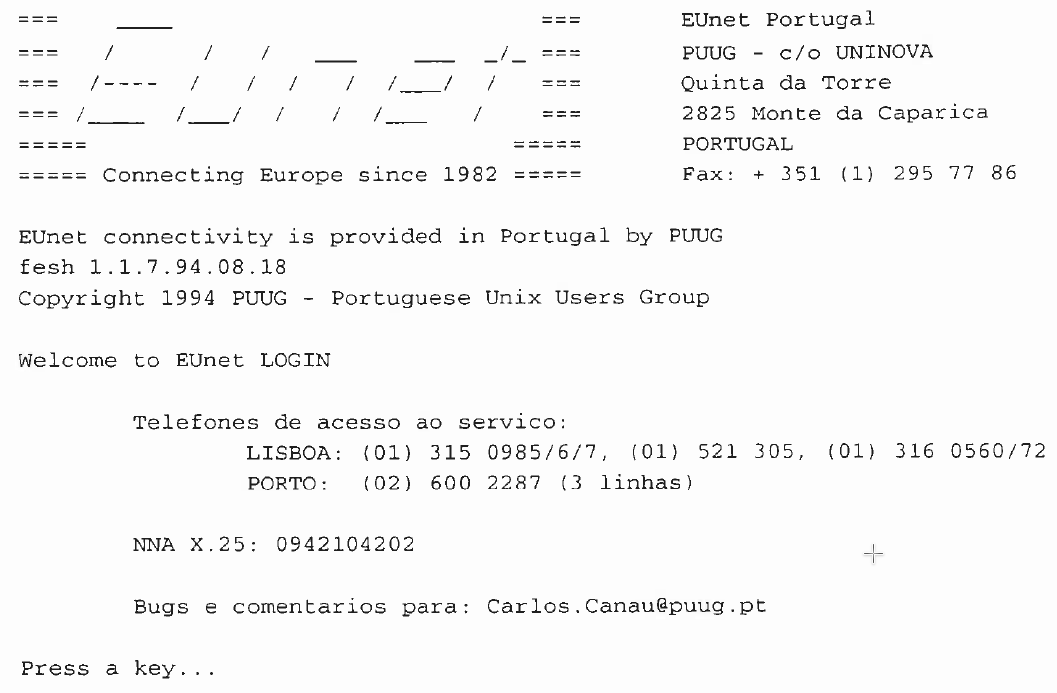
\includegraphics[width=250pt]{EUnet.png}}
\end{frame}

\begin{frame}
\frametitle{Portugal Virtual}
  \begin{itemize}
    \item{} In 1991, LuPa and Goth, who worked on LNEC, found DS9, a text based virtual world hosted in USA
    \item{} Things were a bit different in 1991\ldots
      \begin{itemize}
        \item{} establishing and maintaining a TCP connection to the USA isn't easy, specially taking account the latency
        \item{} the Internet is the world of academics and researchers, ``online'' from 9 to 5
        \item{} knowledge and confort with the English language is\ldots less than now
      \end{itemize}
    \item{} In 1992's Summer, DS9 administrators give their code to their Portuguese friends, so a Portuguese version can be created
    \item{} Cyber Eden (later renamed to Portugal Virtual) is inaugurated in the 1st of October 1992
  \end{itemize}
\end{frame}

\begin{frame}
\frametitle{From Portugal Virtual to Selva Virtual}
  \begin{itemize}
    \item{} the boom of talkers
    \item{} talkers in universities
    \item{} Selva is created in 1998
    \item{} From Selva to Selva V
    \item{} The development of Portugal Virtual
    \item{} Selva and Portugal Virtual merge into Selva Virtual
    \item{} Selva Virtual, the last talker, still evolves
  \end{itemize}
\end{frame}

\begin{frame}
\frametitle{Portugal -- the boom of talkers}
% http://www.rstnd.com/sitesantigos/AEESTV.v1/di/talkers.htm
\center{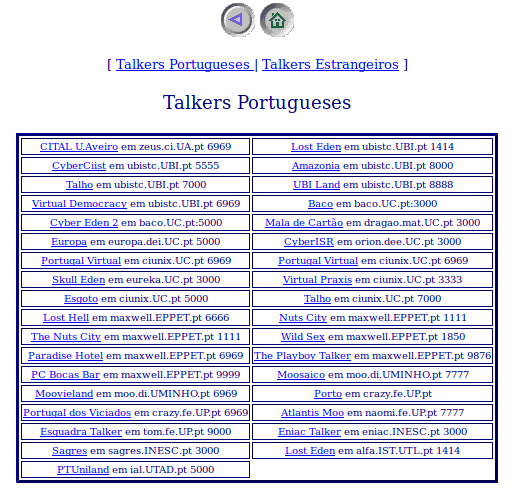
\includegraphics[width=170pt]{talkerspt.png}}
\end{frame}

\begin{frame}
\frametitle{From Portugal Virtual to Selva Virtual}
  \begin{itemize}
    \item{} the boom of talkers
    \item{} talkers in universities
    \item{} Selva is created in 1998
    \item{} From Selva to Selva V
    \item{} The development of Portugal Virtual
    \item{} Selva and Portugal Virtual merge into Selva Virtual
    \item{} Selva Virtual, the last talker, still evolves
  \end{itemize}
\end{frame}

\begin{frame}
\frametitle{Portugal -- talkers in universities}
% http://www.urbi.ubi.pt/000208/_private/ubi_irc.html
\center{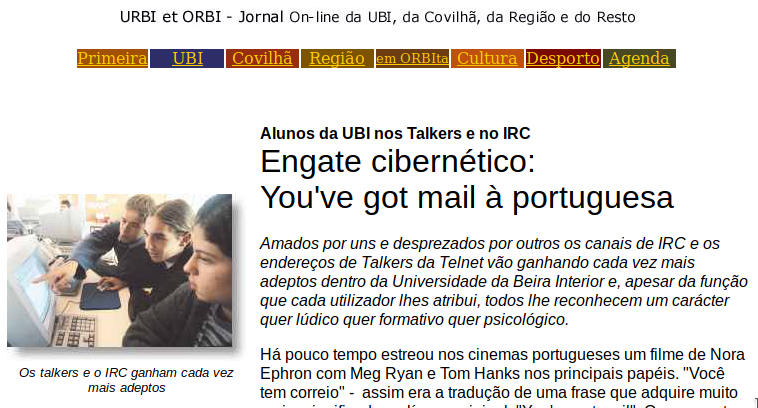
\includegraphics[width=300pt]{URBI-talkers.png}}
\end{frame}

\begin{frame}
\frametitle{From Portugal Virtual to Selva Virtual}
  \begin{itemize}
    \item{} the boom of talkers
    \item{} talkers in universities
    \item{} Selva is created in 1998
    \item{} From Selva to Selva V
    \item{} The development of Portugal Virtual
    \item{} Selva and Portugal Virtual merge into Selva Virtual
    \item{} Selva Virtual, the last talker, still evolves
  \end{itemize}
\end{frame}

\begin{frame}
\frametitle{Portugal -- Selva is created in 1998}
% https://web.archive.org/web/19991018192854/http://student.dei.uc.pt/~smacau/
\center{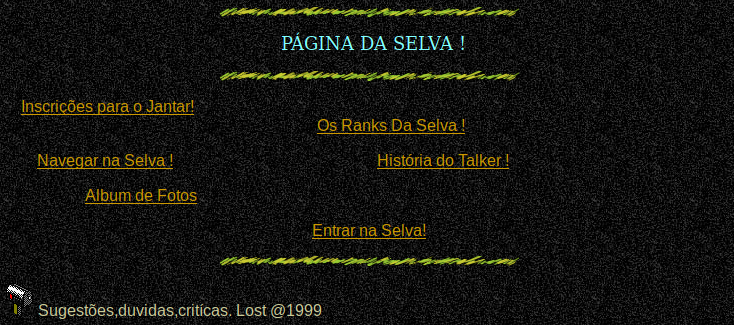
\includegraphics[width=350pt]{selva-web99.png}}
\end{frame}

\begin{frame}
\frametitle{From Portugal Virtual to Selva Virtual}
  \begin{itemize}
    \item{} the boom of talkers
    \item{} talkers in universities
    \item{} Selva is created in 1998
    \item{} From Selva to Selva V
    \item{} The development of Portugal Virtual
    \item{} Selva and Portugal Virtual merge into Selva Virtual
    \item{} Selva Virtual, the last talker, still evolves
  \end{itemize}
\end{frame}

\begin{frame}
\frametitle{Let's try it out!}
  \center{\href{https://selva.grogue.org}{\XeTeXLinkBox{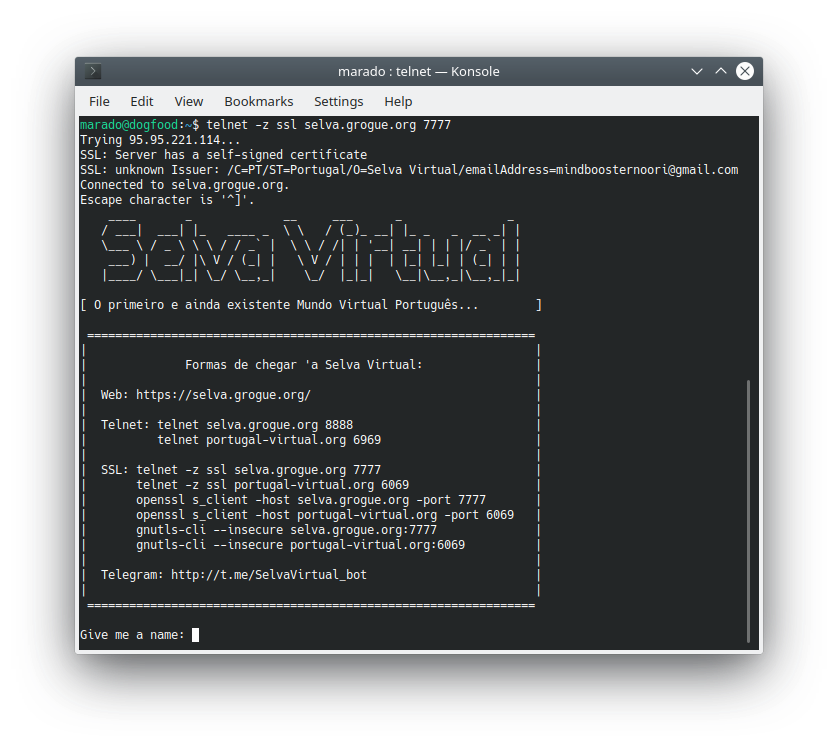
\includegraphics[width=240pt]{selva-login.png}}}}
\end{frame}

\begin{frame}
\frametitle{The color challenge}
% https://en.wikipedia.org/wiki/ANSI_escape_code#3/4_bit
\center{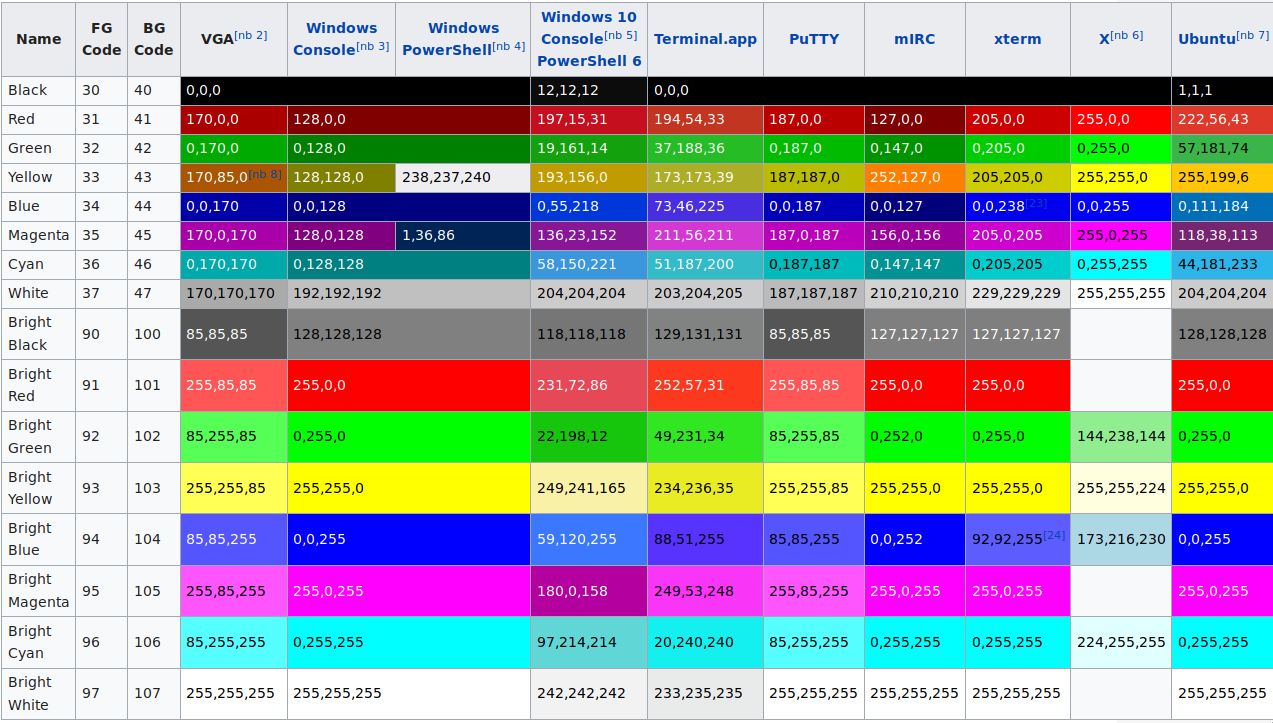
\includegraphics[width=300pt]{ANSI-color.png}}
\end{frame}

\begin{frame}
\frametitle{The security challenge}
% https://en.wikipedia.org/wiki/MUD_client#Protocol_support
\center{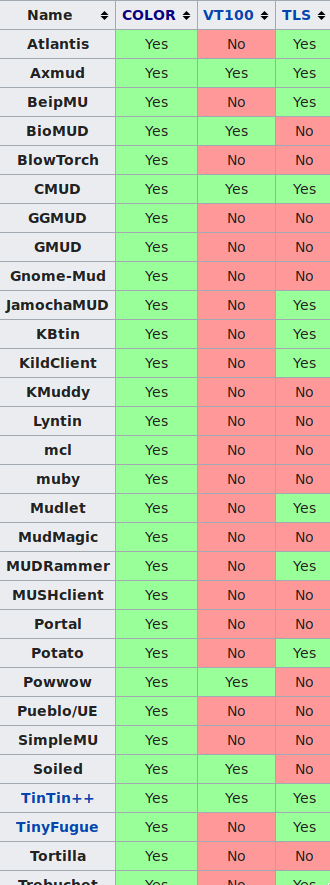
\includegraphics[width=90pt]{TLS-support.png}}
\end{frame}

\begin{frame}
\frametitle{The hosting challenge}
% picture of selva-1 and selva-2 carcasses
\end{frame}

\begin{frame}
\frametitle{The websense challenge}
\end{frame}

\begin{frame}
\frametitle{Current status: hosting}
% picture of the current server
\end{frame}

\begin{frame}
\frametitle{Current status: architecture}
The UNIX way
% graph or description of every component
\end{frame}

\begin{frame}
\frametitle{Current status: user activity}
% .file simultaneo; .file simgraph; .file spod; .file logins; .file nascimentos; .file especies
\end{frame}

\begin{frame}
\frametitle{Current challenges}
% python 3
% TalkerNode
% tg bot
% web client
% article 11 and article 13
% HA
% stunnel and telnet-ssl bugs
\end{frame}

% The next slides are about the future, and there could be more... eg. when
% will we get rid of telnet/insecure connections?

\begin{frame}
\frametitle{Federation: 1988-2018 RIP}
\end{frame}

\begin{frame}
\frametitle{A decentralized future?}
\end{frame}

\begin{frame}
\frametitle{Disclaimer about this presentation}
% screenshot or section of https://bugs.launchpad.net/ubuntu-font-licence/+bug/1167425
\end{frame}

\subtitle{Thank you}
\frame[plain]{\titlepage}

\end{document}
